\chapter{Desarrollo y Resultados}

En este capítulo se detallan los resultados obtenidos en la implementación y
ejecución del presente Proyecto de Grado. En primer lugar, en la Sección \ref{sec:DesRecDat},
se recopilan los datos en \textit{PostgreSQL}.
En segundo lugar, en la Sección \ref{sec:DesProCod}, se procesan los fragmentos 
de código, se crea la firma y se elabora el índice invertido. 
Posteriormente, en la Sección \ref{sec:DesConSisRec}, se crea el Sistema de Recomendación
y se muestran los resultados.

\section{Recopilación de Datos}
\label{sec:DesRecDat}

El peso aproximado de la base de datos de \textit{Stack Overflow} en formato \ac{XML}
es de $50GB$ para el año $2014$. 

\subsection{Obtención de Datos}

La base de datos contiene los siguientes archivos: 

\begin{itemize}
  \item \textit{Badges.xml}
  \item \textit{Comments.xml}
  \item \textit{PostHistory.xml} (\textbf{Ignorado})
  \item \textit{PostLinks.xml}
  \item \textit{Posts.xml} (\textbf{Necesario})
  \item \textit{Tags.xml} (\textbf{Necesario})
  \item \textit{Users.xml}
  \item \textit{Votes.xml}
\end{itemize}

\subsection{Construcción del Esquema}

El \textit{script} inicial recrea la estructura de las siguientes tablas:

\begin{itemize}
  \item \textit{Posts}
  \item \textit{PostCodes}
  \item \textit{PostTags}
  \item \textit{Tags}
\end{itemize}

Se puede encontrar el diagrama \textit{entidad-relación} en el Anexo \ref{ape:diag}.

Luego, los archivos \ac{XML} son procesados
mediante una serie de \textit{scripts} que 
tienen el nombre de la tabla correspondiente.
Estos \textit{scripts} se pueden encontrar en el Anexo \ref{ape:sql}
e incluyen la configuración sugerida para trabajar con
grandes volúmenes de datos.

El archivo \textit{Posts.xml} requiere la creación de la tabla \textit{PostTags},
para representar la relación \textit{many to many}, muchos a muchos,
que la tabla \textit{Post} guarda con respecto a la tabla \textit{Tags}.
Por otro lado, se considera la creación de la tabla \textit{PostCodes},
cuya relación es \textit{one to many}, uno a muchos,
para almacenar los fragmentos de código que son extraídos del tópico.

Estos \textit{scripts} se apoyan sobre la función \textit{xpath}
para extraer los atributos de los elementos y almacenarlos en los campos
correspondientes en su respectiva tabla.

El Fragmento de Código \ref{lst:example}, muestra un ejemplo de uso de la función
\lstinline{xpath()} para extraer el atributo de un elemento.

\begin{lstlisting}[caption={Función xpath.},label={lst:example}]
SELECT unnest(xpath('@Id', '<row Id="1" ... />')) as result;
 result
--------
 1
(1 fila)
\end{lstlisting}

Una vez almacenados los datos, se encuentra que existe un total de $21.736.593$ tópicos,
entre los cuales se consideran solo los que están relacionados con las etiquetas c y c++.
En consecuencia, la cantidad de tópicos utilizados a lo largo del Proyecto de Grado se limita a $1.420.664$.

En la Tabla \ref{tab:topicos} se muestra la cantidad de los tópicos relacionados con las distintas etiquetas.
\begin{table}[h]
\caption{Cantidad de tópicos por etiqueta.}
\label{tab:topicos}
\centering
\begin{tabular}{ccccc}
\hline
{Etiqueta} & {Preguntas} & {Respuestas} & \makecell{Respuestas\\Aceptadas} & {Total} \\
\hline
{todas} & $7.990.786$ & $13.684.117$ & $4.596.859$ & $21.736.593$ \\ 
{c/c++} & $442.450$ & $978.214$ & $284.297$ & $1.420.664$ \\ 
{c++} & $314.869$ & $684.362$ & $203.447$ & $999.231$ \\ 
{c} & $151.856$ & $362.244$ & $96.949$ & $514.100$ \\
\hline
\end{tabular}
\end{table}

Es importante destacar que, tan solo $284.297$ tópicos 
de este conjunto cuentan con una respuesta aceptada,
lo que representa un $29\%$ del total de las preguntas.
La búsqueda se limitaría significativamente si solo estas preguntas fuesen consideradas,
descartando tópicos relevantes para el usuario.

\subsection{Decodificación de Datos}
La decodificación de las entidades especiales 
se realizó empleando la clase \lstinline{StringEscapeUtils},
que contiene las funciones \lstinline{unescapeXml()} y \lstinline{unescapeHtml4()},
las cuales son usadas para decodificar texto en el formato 
\ac{XML} y \ac{HTML} respectivamente.
Esta clase pertenece a la librería mencionada en la Sección \ref{subsec:apache}.

La función \lstinline{unescapeXml()} se emplea para reemplazar
el contenido de los tópicos directamente en la base de datos. 
Mientras que la función \lstinline{unescapeHtml4()},
se utiliza para acceder al cuerpo del tópico.

\subsection{Extracción del Código}

Los fragmentos de código en los tópicos se encuentran bajo las etiquetas \ac{HTML} \lstinline{<pre>} o \lstinline{<code>},
de los cuales solo $773.320$ tópicos cumplen con el formato estándar.

Esto indica que al menos un $54.43\%$ de los tópicos relacionados con c y c++ contienen fragmentos de código,
siendo esta relación mayor en las preguntas ($71.02\%$) y menor en las respuestas ($46.93\%$).

\newpage
Un ejemplo del formato estándar se puede encontrar en el Fragmento de Código \ref{lst:top4},
extraído del tópico con \lstinline{Id = 4}.

\begin{lstlisting}[caption={Tópico Ejemplo.},label={lst:top4}]
...
<pre>
	<code>
		decimal trans = trackBar1.Value / 5000;
		this.Opacity = trans;
	</code>
</pre>
...
\end{lstlisting}

Existe un total de $1.377.716$ fragmentos de código, 
donde el $43.46\%$ se encuentra en las preguntas.
%Esto es un porcentaje importante, pues la cantidad de preguntas representa solo un $31.14\%$ de los tópicos.
%Lo que sugiere una mayor cantidad de fragmentos de código en las preguntas.


La Figura \ref{graf:distribucion} muestra las estadísticas 
descriptivas de los fragmentos de código por tópico,
se encuentra una media de 1 fragmento de código en las preguntas 
y 0 en las respuestas.
Por otra parte, la media es 1 para el total de los tópicos.

\begin{figure}[h]
\centering
\begin{tikzpicture}
\begin{axis}[
boxplot/draw direction=y,
x=2cm,
xtick={1,2,3},
xticklabels={Total, Preguntas, Respuestas},
]
\addplot+ [boxplot prepared={
lower whisker=0,
lower quartile=0,
median=1,
upper quartile=1,
upper whisker=2}
%average=1},
] coordinates {};
\addplot+ [boxplot prepared={
lower whisker=0,
lower quartile=0,
median=1,
upper quartile=2,
upper whisker=4}
%average=1},
] coordinates {};
\addplot+ [boxplot prepared={
lower whisker=0,
lower quartile=0,
median=0,
upper quartile=1,
upper whisker=2}
%average=0},
] coordinates {};
% \addplot+ [boxplot prepared={
% lower whisker=1,
% lower quartile=1,
% median=1,
% upper quartile=2,
% upper whisker=31},
% ] coordinates {};
% \addplot+ [boxplot prepared={
% lower whisker=1,
% lower quartile=1,
% median=1,
% upper quartile=2,
% upper whisker=42},
% ] coordinates {};
\end{axis}
\end{tikzpicture}
\caption{Estadísticas descriptivas de los fragmentos de código.}
\label{graf:distribucion}
\end{figure}


Se aprecia que la cantidad de líneas en los fragmentos de código pertenecientes a las preguntas suele ser mayor,
esto se evidencia al analizar la Figura \ref{graf:lineas}.
Donde se muestra una media de 8 líneas de código en las preguntas y 4 en las respuestas,
mientras que la media general es 5.

\begin{figure}[h]
\centering
\begin{tikzpicture}
\begin{axis}[
boxplot/draw direction=y,
x=2cm,
xtick={1,2,3},
xticklabels={Total, Preguntas, Respuestas},
]
\addplot+ [boxplot prepared={
lower whisker=1,
lower quartile=2,
median=5,
upper quartile=14,
upper whisker=31},
%upper whisker=1266},
] coordinates {};
\addplot+ [boxplot prepared={
lower whisker=1,
lower quartile=3,
median=8,
upper quartile=19,
upper whisker=42},
%upper whisker=1266},
] coordinates {};
\addplot+ [boxplot prepared={
lower whisker=1,
lower quartile=1,
median=4,
upper quartile=10,
upper whisker=23},
%upper whisker=1236},
] coordinates {};
\end{axis}
\end{tikzpicture}
\caption{Estadísticas descriptivas de las líneas de código.}
\label{graf:lineas}
\end{figure}


\section{Procesamiento del Código}
\label{sec:DesProCod}

Como han indicado \cite{monperrus:hal-00987395},
el motor de búsqueda de \textit{Stack Overflow} no es adecuado para realizar consultas utilizando fragmentos de código.
Debido a esto, se aplicó la técnica de \ac{LSH} para crear un índice especializado.

\subsection{Representación Intermedia del Código}
\label{subsec:DesIntCod}

Antes de transformar el código, se debe tener algunas consideraciones en cuenta:

\begin{itemize}
  \item Existen caracteres reservados en el formato \ac{HTML}, que deben ser decodificados.
  Algunos de estos son: \lstinline{&amp;}, \lstinline{&nbsp;}, \lstinline{&#64;}.

  \item Se deben eliminar todas las directivas de preprocesamiento, no son significativas.
  Como por ejemplo: \lstinline{#include <cstring>}.
  
  \item No es necesario preocuparse por los comentarios, el \textit{lexer} se encargará de ellos.
  Tal es el caso de: \lstinline{// This is a valid comment}.
\end{itemize}

El \textit{lexer} se encarga de identificar los lexemas como enteros en el rango de $1$ a $144$.
Se encontró que la mitad de ellos no se usan, ya que son asignados por el \textit{paser}
o han sido marcados como obsoletos. Una lista detallada de estos lexemas
puede consultarse en el Anexo \ref{ape:tok}.

\newpage
El \textit{lexer} identifica los lexemas en el Fragmento de Código \ref{lst:fc4} 
y los separa en una serie de \textit{tokens} de la siguiente manera:

\begin{verbatim}
 identifier, identifier, assign, identifier, dot, identifier, div, integer,
        semi, identifier, dot, identifier, assign, identifier, semi
\end{verbatim}

\begin{lstlisting}[caption={Fragmento de código en c++},label={lst:fc4}]
decimal trans = trackBar1.Value / 5000;
this.Opacity = trans;
\end{lstlisting}
Estos \textit{tokens} son representados por enteros, tal que:

\begin{verbatim}
             1, 1, 38, 1, 50, 1, 52, 2, 5, 1, 50, 1, 38, 1, 5
\end{verbatim}

Luego, se utiliza la técnica de \textit{n-grams} sobre el Fragmento de Código
\ref{lst:fc4} con $n = 4$, ya que ha mostrado los mejores resultados~\cite{Burrows:2007:EPD:1228662.1228664}.
Obteniéndose la siguiente secuencia:

\begin{verbatim}
(1,1,38,1), (1,38,1,50), (38,1,50,1), (1,50,1,52), (50,1,52,2), (1,52,2,5),
 (52,2,5,1), (2,5,1,50), (5,1,50,1), (1,50,1,38), (50,1,38,1), (1,38,1,5)
\end{verbatim}

Posteriormente, se suele usar una función de \textit{hash}
para transformar la secuencia de \textit{n-grams} en una secuencia de enteros.
Sin embargo, dada la naturaleza de estos \textit{n-grams}, 
se pueden almacenar sus valores en enteros sin colisiones;
dado a que existen $429.981.695$ combinaciones
en el conjunto de los \textit{4-grams}, al que se denomina $G$.

Luego, como $G$ es finito, es un conjunto numerable; 
por lo tanto, existe una función $f$ inyectiva al conjunto de los naturales, tal que:
\begin{equation*}
f : G \rightarrow\mathbb{N}
\end{equation*}
Tal función se escribe:
\begin{equation*}
f(G) = (G_3-1) * 144^3 + (G_2-1) * 144^2 + (G_1-1) * 144^1 + (G_0-1)*144^0
\end{equation*}

%Por ejemplo, al representar el \textit{} $(1,1,38,1)$ como un entero, se tiene:

%\begin{equation*}
%5328 = (1-1) * 144^3 + (1-1) * 144^2 + (38-1) * 144^1 + (1-1)*144^0
%\end{equation*}

Luego, para el Fragmento de Código \ref{lst:fc4} se obtiene la siguiente representación:

\begin{verbatim}

  5328, 767281, 110488464, 1016115, 146320561, 1057684, 152306496, 3068977,
               11950992, 1016101, 146318544, 767236, 110482127
\end{verbatim}

\subsection{Creación de la Firma del Código}
\label{subsec:DesFirCod}

Se escogen $100$ funciones de \textit{hash} para la elaboración
de la firma mediante la técnica de \textit{MinHash},
tal que el error esperado es a lo sumo un $10\%$.
Continuando con el Fragmento de Código \ref{lst:fc4} que usamos como ejemplo,
se procede a generar la firma.

Se escogen las siguientes funciones de \textit{hash}:
\begin{gather*}
f_1(x) = (x * 133 + 2.163) \bmod 429.981.701 \\
f_2(x) = (x * 140.002 + 1.234) \bmod 429.981.701\\
\vdots \\
f_{100}(x) = (x * 91.231.268 + 300.122.522) \bmod 429.981.695
\end{gather*}
	
%A su vez, se escogen los coeficientes $a=140.002$ y $b=1.234$, se tiene:

%\begin{equation*}
%f_2(x) = (x * 140.002 + 1.234) \bmod 429.981.701
%\end{equation*}

%\begin{equation*}
%\vdots
%\end{equation*}

%Finalmente, se escogen los coeficientes $a = 91.231.268$ y $b = 300.122.522$, se tiene:

%\begin{equation*}
%f_{100}(x) = (x * 91.231.268 + 300.122.522) \bmod 429.981.695
%\end{equation*}

Al aplicar estas funciones de \textit{hash} sobre el Fragmento de Código \ref{lst:fc4}, se obtienen los valores:
\begin{gather*}
f_1(x) \rightarrow \{604227, 86704916, 15729266, 114823158, 194920918, 119520455,\\
							  11368171, 346796564, 60519156, 114821576, 194692997, 86699831, 15013185\}\\
f_2(x) \rightarrow \{315950189, 355432247, 14244687, 364172134, 412965015, 164171458,\\
							  421501636, 111199889, 103984627, 362212106, 130580981, 349132157, 416997116\}\\
\vdots\\
f_{100}(x) \rightarrow \{181460756, 87946214, 32252656, 301023389, 176237545, 260167737,\\
									 323195011, 209406491, 271127092, 17027248, 139482376, 127203813, 324373383\}
\end{gather*}

Luego, la firma para el Fragmento de Código \ref{lst:fc4} estaría conformada por los mínimos:
\begin{gather*}
firma(C_1) = (604227, 14244687, \dots, 17027248)
\end{gather*}

En el proceso se descartó $48.028$ fragmentos nulos, persistiendo $1.329.688$.
De los cuales, $581.798$ se asocian con preguntas y $747.890$ se asocian con respuestas.

\subsection{Construcción de un Índice}
\label{subsec:DesConInd}

La configuración inmediata para el \ac{LSH} consiste en dividir las
firmas cuyo tamaño es $100$, en $20$ bandas con $5$ filas cada una.
Esto da como resultado un umbral de similitud aproximado del $54.93\%$,
que los fragmentos de código tienen que superar para convertirse en pares candidatos.

La creación del índice produjo un total de $26.593.760$
entradas en la base de datos, las cuales se distribuyen entre las bandas.
Cada banda está conformada por $1.329.688$ minifirmas,
que se emplean como claves y se asocian a un fragmento de código.

\subsubsection{Evaluación del Índice Invertido}

Para comprobar la funcionalidad del índice,
se escogió un total de $1.000$ fragmentos de código escogidos al azar de forma uniforme,
los cuales fueron extraídos directamente de la base de datos y
se identifican como conjunto $1$. Este conjunto se puede consultar en el Anexo \ref{ape:conj}.


\begin{itemize}
  \item $1.000/1.000$ tópicos encontrados.
  \item $730/1.000$ tópicos encontrados en el primer lugar.
  \item $122/1.000$ tópicos encontrados entre los diez primeros.
  \item $148/1.000$ tópicos encontrados en alguna otra posición.
\end{itemize}

Las pruebas realizadas sobre el conjunto $1$,
se usan para evaluar la efectividad al seleccionar un tópico.
Los resultados muestran que cualquier fragmento de código indexado correctamente,
es considerado par candidato y por consiguiente encontrado.

Se utilizan las firmas para evaluar la similitud entre los fragmentos de código,
todos los fragmentos se evaluaron con una similitud del $100\%$.
Si se usa el coeficiente de similitud de \textit{Jaccard} para comparar los fragmentos los resultados apenas varían,
modificando un solo tópico; el tópico modificado pasaría del 2\textsuperscript{do} al 1\textsuperscript{er} lugar,
debido a que un tópico similar que se encontraba en la primera posición dejo de tener una similitud del 100\%.

Las pruebas realizadas arrojaron datos estimados del tiempo de búsqueda,
cuyo promedio es $194$ milisegundos. Gran parte del tiempo es invertido
en la consulta realizada, cuyo promedio es $185$ milisegundos.
Son encontrados $500$ pares candidatos en promedio y
el tiempo empleado para evaluar cada firma es de $0.28$ milisegundos aproximadamente.



%La certeza de cuán parecidos son los fragmentos de código, es obtenida a través del \textit{MinHash}.
%Lo que implica que dos fragmentos cualesquiera, cuya estructura sea idéntica, 
%tendrán la misma ponderación al ser comparados con un tercer fragmento.
%Por lo tanto, el orden en el que aparecen los fragmentos de código estructuralmente iguales, es arbitrario.

Para evaluar la capacidad de búsqueda de fragmentos de código arbitrario,
se utilizó un conjunto de  $195$ fragmentos extraidos de una fuente externa,
al que se identifica como conjunto $2$. El origen de este conjunto se especifica en el Anexo \ref{ape:conj}.

Estos fragmentos de código no guardan relación con la base de datos de \textit{Stack Overflow} y
se utilizan para determinar la viabilidad al realizar consultas con fragmentos arbitrarios.

Se estableció una clasificación basada en la similitud estructural de los fragmentos de código.
Aquellos fragmentos de código cuya similitud es igual o superior
al $95\%$, se clasifican en el rango $1$, si es igual o superior
al $85\%$, se clasifican en el rango $2$, si es igual o superior
al $70\%$, se clasifican en el rango $3$ y si es igual o superior
al $50\%$, se clasifican en el rango $4$.
 
Los resultados encontrados al aplicar esta clasificación al conjunto de
fragmentos de código arbitrario, se encuentran en la Tabla \ref{tab:clasificacion}.

\begin{table}[h]
\caption{Clasificación de Fragmentos de Código.}
\label{tab:clasificacion}
\centering
\begin{tabular}{ccccc}
\hline
{Rango 1} & {Rango 2} & {Rango 3} & {Rango 4} & {Sin rango} \\
\hline
$12$ & $8$ & $20$ & $55$ & $100$ \\
\hline
\end{tabular}
\end{table}

A continuación, se detallan las características encontradas en cada rango:

\begin{description}
  \item [Rango 1] Son fragmentos de código considerados estructuralmente iguales.
  Pueden haber variaciones en la cardinalidad de los \textit{n-gram}.
  Esto se traduce, en secuencias de tamaño $n$ repetidas.
  \item [Rango 2] Son fragmentos de código con inserciones de una o más constantes,
  variables u operadores que modifican pocos \textit{n-gram}, típicamente de $3$ a $7$.
  \item [Rango 3] Son fragmentos de código que poseen cambios estructurales básicos,
  dependiendo de la longitud del código se muestran en mayor o menor grado.
  \item [Rango 4] Son fragmentos de código que poseen cambios estructurales importantes,
  en general difieren mucho del fragmento de código considerado.
  \item [Sin rango] Son fragmentos de código con muy poca o ninguna similitud.
\end{description}

A efectos de la evaluación de los fragmentos de código se define la especificidad
de un fragmento de código, como la cantidad de líneas de código que éste posee.
Sin definir una cantidad precisa, se dirá que a mayor especificidad, mayor cantidad de líneas de código.

La Figura \ref{graf:lineas2} muestran un crecimiento lineal en el conjunto $2$,
que involucra a los fragmentos código del rango $2$ en adelante.
Dicho comportamiento sugiere que la especificidad de los fragmentos de código,
disminuye la probabilidad de encontrar otros fragmentos estructuralmente iguales o similares.

\begin{figure}[h]
\centering
\begin{tikzpicture}
\begin{axis}[
boxplot/draw direction=y,
x=2cm,
xtick={1,2,3,4,5},
xticklabels={Rango1, Rango2, Rango3, Rango4, SinRango},
]
\addplot+ [boxplot prepared={
lower whisker=2,
lower quartile=7,
median=8,
upper quartile=10.5,
upper whisker=15},
] coordinates {};
\addplot+ [boxplot prepared={
lower whisker=3,
lower quartile=7,
median=7.5,
upper quartile=10.5,
upper whisker=12},
] coordinates {};
\addplot+ [boxplot prepared={
lower whisker=4,
lower quartile=10,
median=12.5,
upper quartile=18.5,
upper whisker=23},
%upper whisker=34},
] coordinates {};
\addplot+ [boxplot prepared={
lower whisker=6,
lower quartile=15,
median=22,
upper quartile=31,
upper whisker=45},
] coordinates {};
\addplot+ [boxplot prepared={
lower whisker=1,
lower quartile=22.5,
median=31,
upper quartile=38,
upper whisker=51},
] coordinates {};
\end{axis}
\end{tikzpicture}
\caption{Estadísticas descriptivas de las líneas de código.}
\label{graf:lineas2}
\end{figure}

Se hace notar que los fragmentos de código que se encuentran en el rango $2$ y posterior,
no tienen una estructura equivalente dentro de la base de datos.
Esto se desprende de las pruebas realizadas sobre el conjunto $1$,
donde todos los fragmentos de código se corresponden al rango $1$.

Sin embargo, existen muchos más fragmentos de código en el rango $1$ que en el rango $2$.
Lo que sugiere que una media de 8 líneas de código es lo apropiado para 
encontrar estructuras equivalentes dentro de la base de datos.

Luego, al evaluar los fragmentos de código en el rango $8\pm1$, se encuentran solo 16 fragmentos
y como se evidencia en la Tabla \ref{tab:clasificacion2}, la probabilidad de que un fragmento
con 8 líneas de código se encuentre en el rango $1$ es de $37.5\%$, en el rango $2$ es
de $25.0\%$, en el rango $3$ es de $18.75\%$, en el rango $4$ es de $6.25\%$ y no tenga rango
es de $12.5\%$ para el conjunto $2$.

\begin{table}[h]
\caption{Clasificación de Fragmentos de Código en el rango $8\pm1$.}
\label{tab:clasificacion2}
\centering
\begin{tabular}{ccccc}
\hline
{Rango 1} & {Rango 2} & {Rango 3} & {Rango 4} & {Sin rango} \\
\hline
$6$ & $4$ & $3$ & $1$ & $2$ \\
\hline
\end{tabular}
\end{table}

\section{Sistema de Recomendación}
\label{sec:DesConSisRec}

El Sistema de Recomendación propuesto se implementa como
un \textit{plug-in} de \textit{Eclipse}, que se comunica mediante
un esquema \textit{cliente-servidor} y realiza consultas directamente
al servidor de base de datos \textit{PostgreSQL}.
Este proceso se muestra en la Figura \ref{fig:diag1}.

\begin{figure}[h]
\centering
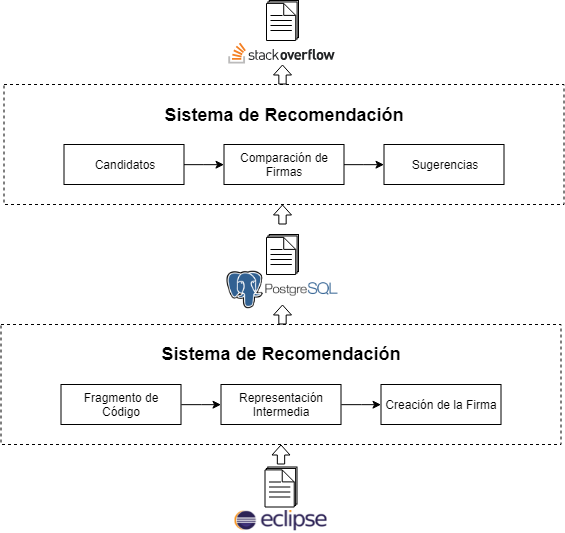
\includegraphics[width=30em]{img/comunicacion.png}
\caption{Estructura de Comunicación}
\label{fig:diag1}
\end{figure}

\subsection{Establecer Comunicación}

El Sistema de Recomendación 
captura el fragmento de código provisto por el usuario y sigue los pasos 
establecidos en las secciones: Sección \ref{subsec:DesIntCod} y Sección \ref{subsec:DesFirCod}.
Entonces, el fragmento de código es transformado en una serie de \textit{tokens}
mediante el \textit{lexer}, los cuales son agrupados para formar \textit{4-grams}
y se calcula la firma a partir de ellos.
%Entonces, la clase \textit{Tokenizer} recibe el fragmento de código 
%y lo pasa al \textit{lexer}, retornando un \textit{iterador}.
%El \textit{iterador} es recorrido obteniendo una serie de \textit{tokens},
%los cuales son agrupados para formar \textit{4-grams} y se calcula el valor de
%cada uno mediante la clase \textit{Ngram}, produciendo un conjunto de enteros;
%ésta es la Representación Intermedia del código.
%La clase \textit{MinHash} recibe el conjunto de enteros y
%genera la firma con los mínimos obtenidos al multiplicar las funciones de \textit{hash}.
Luego, el Sistema de Recomendación construye la consulta con la firma obtenida 
y la envía al servidor de bases de datos.

Posteriormente, el servidor de bases de datos recibe la consulta y separa
la firma en minifirmas. Se usa el índice invertido, desarrollado en la
Sección \ref{subsec:DesConInd}, para buscar los pares candidatos
mediante las minifirmas. Luego, se forma una lista con los pares candidatos
encontrados que incluye sus firmas y el servidor la envía al cliente.

Finalmente, el cliente recibe la lista y compara las firmas. De esta manera,
construye las sugerencias en base a la similitud de los pares candidatos,
mostrando solo aquellos que cumplen con los parámetros establecidos.


\subsection{Determinar Tipos de Consulta}

Las sugerencias realizas se pueden limitar a un subconjunto especifico 
de tópicos, entre los cuales se encuentran las preguntas y las respuestas.
A su vez, la consulta de preguntas puede ser restringida a aquellas
que tengan una respuesta aceptada, mientras que la consulta de respuestas
puede ser restringida a aquellas que han sido aceptadas.

En la Sección \ref{subsec:DesConInd}, se estableció una clasificación
en base a la similitud de los fragmentos de código, que describe las
características de cada rango. Esta clasificación es empleada
para filtrar los resultados mostrados en las sugerencias.

El orden por defecto en el que se muestran los tópicos está dado
por la similitud de los fragmentos de código que éstos contienen.
Sin embargo, es posible ordenar la lista de sugerencias en base
a la reputación de los tópicos.

\subsection{Interfaz del Usuario}

El Sistema de Recomendación se provee con una interfaz
sencilla, compuesta de tres elementos describen a continuación.
La Figura \ref{fig:srse} muestra dicha interfaz.

El botón de consulta dispara un evento que captura
el fragmento de código resaltado por el usuario,
inmediatamente se muestra la ventana de consulta.

La ventana de consulta permite especificar los 
parámetros de búsqueda, entre los que se encuentran:
los filtros a aplicar sobre los tópicos, 
las categorías en las que se hallan
y el orden en el que se muestran.
%Esta ventana contiene un botón para enviar
%y otro para cancelar.

La ventana de sugerencias muestra la lista de
los tópicos de \textit{Stack Overflow} propuestos.
Se compone del tipo del tópico, el título,
la reputación y el porcentaje de similitud.

\begin{figure}[h]
\centering
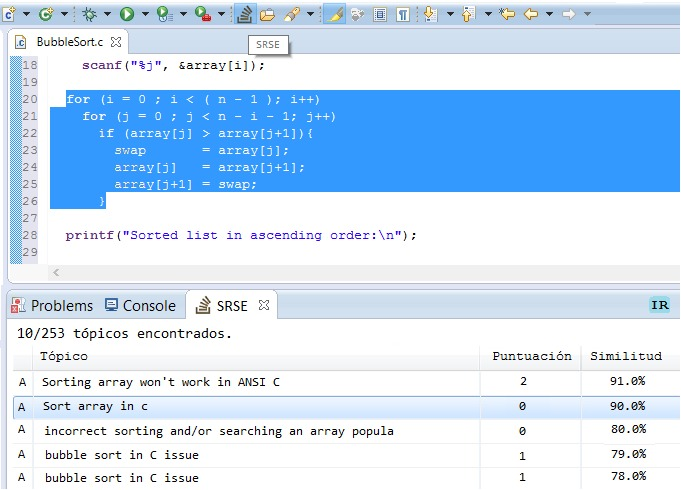
\includegraphics[width=30em]{img/srse.jpg}
\caption{Interfaz del Usuario}
\label{fig:srse}
\end{figure}

% \subsection{Ejemplo de uso}


% Si tomamos una implementación típica, como lo es \textit{bubble sort},
% que se muestra en la Figura \ref{lst:bubble} obtendremos como sugerencias,
% los resultados que se muestran en la Figura \ref{lst:rbubble}.

% \begin{lstlisting}[caption={Bubble Sort.},label={lst:bubble}]
% for (c = 0 ; c < ( n - 1 ); c++)
	% for (d = 0 ; d < n - c - 1; d++) {
		% if (array[d] > array[d+1]) {
			% swap       = array[d];
			% array[d]   = array[d+1];
			% array[d+1] = swap;
		% }
% \end{lstlisting}

% \begin{lstlisting}[caption={Resultados Bubble Sort.},label={lst:rbubble}]
% 1) A:Sorting array won't work in ANSI C (2) 91.0%
% 2) A:Sort array in c (0) 90.0%
% 3) A:incorrect sorting and/or searching an array popula (0) 80.0%
% 4) A:bubble sort in C issue (0) 79.0%
% 5) A:bubble sort in C issue (1) 78.0%
% 6) A:bubble sort in C issue (1) 77.0%
% 7) A:Sorting gives inconsistent results, due to loop bo (0) 75.0%
% 8) A:Recursive Bubble Sort in C (1) 73.0%
% 9) Q:Time Computational complexity? (-3) 73.0%
% 10) Q:Undefined behaviour while swapping/exchanging poin (0) 71.0%
% \end{lstlisting}

% Si en cambio, seleccionamos la implementación completa de \textit{bubble sort}
% como se muestra en la Figura \ref{lst:bubblec} obtendremos como sugerencias,
% los resultados que se muestran en la Figura \ref{lst:rbubblec}.

% \begin{lstlisting}[caption={Bubble Sort Completo.},label={lst:bubblec}]
% void main() {
	% int array[100];
	% int i, j, n, swap;
	% scanf("%d", &n); // Enter number of elements
	% for (i = 0; i < n; i++) // Enter integers
		% scanf("%d", &array[i]);
	% for (i = 0; i < n - 1; i++)
		% for (j = 0 ; j < n - i - 1; j++) {
			% if (array[j] > array[j+1]) {
				% swap       = array[j];
				% array[j]   = array[j+1];
				% array[j+1] = swap;
			% }
	% for (i = 0; i < n; i++) // Print ordered list
		% printf("%d\n", array[i]);
% }
% \end{lstlisting}

% \begin{lstlisting}[caption={Resultados Bubble Sort completo.},label={lst:rbubblec}]
% 45 resultados encontrados.
% 1) Q:I made this program for sorting of n numbers in C, (0) 71.0%
% 2) Q:warning: comparison between pointer and integer an (2) 68.0%
% 3) Q:The program wont work for n>9... It works fine whe (0) 67.0%
% 4) Q:Unable to run this code still it shows no errors? (0) 67.0%
% 5) Q:Can't find most frequent word (3) 65.0%
% 6) Q:What's wrong with my for-loop? (1) 65.0%
% 7) Q:Calculating a Percentile (1) 61.0%
% 8) A:Bubble Sort in C (2) 61.0%
% 9) Q:Merge 2 arrays and omit all repeating elements (0) 61.0%
% 10) Q:adding an extra number to be sorted (0) 61.0%
% \end{lstlisting}

\subsection{Evaluación del Sistema de Recomendación}

Se seleccionó un conjunto de 10 elementos, llamado conjunto 3,
que contiene algoritmos de variado propósito,
la prueba cumple con las siguientes condiciones:

\begin{itemize}
	\item Algoritmos completos seleccionados al azar.
	\item Se verifican solo los 10 primeros resultados.
	\item Se verifican solo si su similitud es mayor al 50.\%.
	\item El resultado de los tópicos se clasifica en 3 áreas, encontrado, relacionado, no encontrado;
	para alguno de los tópicos en ese orden.
\end{itemize}

\begin{lstlisting}[caption={Alexander Bogomolny.},label={lst:alex}]
3 resultados encontrados.
1) A:All possible combinations of n items selected rand (0) 83.0%
2) A:Creating every possible value of a fixed size arra (0) 83.0%
3) A:Generating all size k subsets of {0, 1, 2, ... n-1 (1) 53.0%
\end{lstlisting}

\newpage
\begin{lstlisting}[caption={Bin Packing.},label={lst:binpack}]
6 resultados encontrados.
1) Q:Read and Display matrix (0) 55.0%
2) Q:"for" loop inside a switch case doesn't work (0) 53.0%
3) A:Prime number generation algorithm (-2) 52.0%
4) Q:returning a floating point value from a function (1) 51.0%
5) Q:nth root of a number (6) 50.0%
6) Q:Segmentation Fault Error; Absolute Value Table (0) 50.0%
\end{lstlisting}

\begin{lstlisting}[caption={Binary Search Tree.},label={lst:binsearch}]
47 resultados encontrados.
1) Q:errors in delete function of binary search tree (-1) 64.0%
2) Q:AddNew Function using Linked List In C (0) 60.0%
3) Q:Getting error in deleting a node in a linked list  (0) 59.0%
4) Q:Nested Functions are disabled, use -fnested-functi (-2) 57.9%
5) Q:segmentation fault while implementing the binary t (-1) 56.9%
6) Q:Printing Reversed linked list iteratively (3) 56.0%
7) Q:Showing Error Segmentation fault (-7) 56.0%
8) Q:C Program to copy one binary search tree to anothe (1) 56.0%
9) Q:Write a function in c with which we can add more t (-1) 56.0%
10) Q:Binary search tree Segfault (-1) 56.0%
\end{lstlisting}

\begin{lstlisting}[caption={Fisher Yates.},label={lst:yates}]
2 resultados encontrados.
1) A:Is this C implementation of Fisher-Yates shuffle c (22) 63.0%
2) Q:Shuffle a struct (2) 63.0%
\end{lstlisting}

\begin{lstlisting}[caption={Knapsack Problem.},label={lst:knapsack}]
1 resultados encontrados.
1) Q:Knapsack 1/0 Implementation needs explanation (0) 94.0%
\end{lstlisting}

\newpage
\begin{lstlisting}[caption={Selection Sort.},label={lst:selec}]
6 resultados encontrados.
1) A:array in descending order doesn't work in C (4) 68.0%
2) A:C Sorting an array by integer (1) 61.0%
3) Q:Passing an array as an argument to a function poin (0) 54.0%
4) Q:trouble reading a 2D array of characters in C? (0) 51.0%
5) Q:Factorial -C (Linux) (1) 50.0%
6) Q:How to check if the elements in the main diagonal  (0) 50.0%
\end{lstlisting}

\begin{lstlisting}[caption={The Sieve of Eratosthenes.},label={lst:sieve}]
2 resultados encontrados.
1) Q:The Sieve of Eratosthenes code in C (0) 78.0%
2) Q:Dynamic memory array crash the executable (1) 53.0%
\end{lstlisting}

Los resultados obtenidos se muestran en la Tabla \ref{tab:res3},
junto con el número de líneas,
la cantidad de candidatos y
el mayor porcentaje obtenido.

\begin{table}[h]
\caption{Resultados conjunto C.}
\label{tab:res3}
\centering
\begin{tabular}{ccccc}
\hline
{Algoritmo} & {Resultado} & {Líneas} & {Candidatos} & {Porcentaje} \\
\hline
Alexander Bogomolny & $Encontrado$ & $36$ & $3$ & $83\%$ \\
Bin Packing & $No encontrado$ & $30$ & $6$ & $55\%$ \\
Binary Search Tree & $Encontrado$ & $163$ & $47$ & $64\%$ \\
Fibonacci Search & $No Encontrado$ & $48$ & $0$ & $0\%$ \\
Fisher Yates & $Encontrado$ & $33$ & $2$ & $63\%$ \\
Hash Table & $No Encontrado$ & $184$ & $0$ & $0\%$ \\
0-1 Knapsack Problem & $Encontrado$ & $78$ & $1$ & $94\%$ \\
Naor Reigngold & $No Encontrado$ & $17$ & $0$ & $0\%$ \\
Selection Sort & $Encontrado$ & $41$ & $6$ & $68\%$ \\
Sieve Eratosthenes & $Encontrado$ & $22$ & $2$ & $78\%$ \\
\hline
\end{tabular}
\end{table}

Se confirman varios aspectos resaltados en la Sección \ref{subsec:DesConInd}.
En primer lugar, si existen estructuras equivalentes o idénticas, 
el Sistema de Recomendación las encuentra.
Lo que se puede apreciar en el resultado obtenido por el código \textit{0-1 Knapsack Problem},
cuya especificidad es alta, tiene un gran porcentaje de similitud y es el único encontrado.
En segundo lugar, la especificidad disminuye la probabilidad de encontrar fragmentos de código similares.
Lo que se desprende de los resultados obtenidos por el código \textit{Tabla de Hash} y el código \textit{Binary Search Tree},
implementaciones que suelen ser muy comunes y sin embargo, solo fue posible encontrar uno de ellos.

En la Tabla \ref{tab:resss3} se muestran los resultados finales obtenidos,
se aprecia una efectividad del $60.0\%$ al evaluar códigos completos.
Sin embargo, estos códigos son muy comunes y se espera que el porcentaje 
baje ante una implementación propia.

\begin{table}[H]
\caption{Resultados Conjunto 3}
\label{tab:resss3}
\centering
\begin{tabular}{ccc}
\hline
{Resultado} & {Cantidad} & {Porcentaje} \\
\hline
$Encontrado$ & $6$ & $60.0\%$ \\
$No Encontrado$ & $4$ & $40.0\%$ \\
$Relacionado$ & $0$ & $0.0\%$ \\
\hline
\end{tabular}
\end{table}

